\documentclass[11pt,a4paper]{article}
\usepackage[utf8x]{inputenc}
\usepackage[T1]{fontenc}
\usepackage{mathptmx}
\usepackage{graphicx}
\usepackage[pdftex,linkcolor=black,pdfborder={0 0 0}]{hyperref} % Format links for pdf
\usepackage{calc} % To reset the counter in the document after title page
\usepackage{enumitem} % Includes lists
\usepackage{caption}
\captionsetup[figure]{font=small,labelfont=small,labelfont=bf}
\usepackage{subcaption}
\usepackage{amsmath}
\usepackage{fancyvrb,newverbs,xcolor}
\usepackage{verbatim}

\definecolor{cverbbg}{gray}{0.93}

\newenvironment{lcverbatim}
 {\SaveVerbatim{cverb}}
 {\endSaveVerbatim
  \flushleft\fboxrule=0pt\fboxsep=.5em
  \colorbox{cverbbg}{%
    \makebox[\dimexpr\linewidth-2\fboxsep][l]{\BUseVerbatim{cverb}}%
  }
  \endflushleft
}

\renewcommand\thesection{Task \arabic{section}}
\renewcommand\thesubsection{\alph{subsection}.)}
\renewcommand\thesubsubsection{\Roman{subsubsection}:}

\frenchspacing
\linespread{1.2}
\usepackage[a4paper, lmargin=0.12\paperwidth, rmargin=0.12\paperwidth, tmargin=0.05\paperheight, bmargin=0.1\paperheight]{geometry}

\usepackage[all]{nowidow} % Tries to remove widows
\usepackage[protrusion=true,expansion=true]{microtype}

\title{Exercise 1}
\author{Kai Schneider}
\date{\today}

\begin{document} 

\maketitle

\section{}

\subsection{}

$k = 2$, $\epsilon=0.5$ \newline
$\rightarrow P(\textrm{greedy})=1-\epsilon+\frac{\epsilon}{k}=1-0.5+\frac{0.5}{2}=0.75$ \newline
$\rightarrow P(\textrm{non-greedy})=\frac{\epsilon}{k}=\frac{0.5}{2}=0.25$

\subsection{}

$k=4 \; \rightarrow a_{i} \; \textrm{with} \; i=1:4$,  $\; Q_{1}(a_{i})=0$ \newline
with $A_{t}=\underset{a}{\operatorname{argmax}}Q_{t}(a)$ as the greedy policy and 
$Q_{t}(a)=\frac{\sum\limits_{i=1}^{t-1} R_{i,a_{i}=a}}{n(a)}$ and the given data:\newline

\begin{align*}
    A_{1}=1 \;\;\;\;\;\; & R_{1}=1 \\
    A_{2}=2 \;\;\;\;\;\; & R_{2}=1 \\
    A_{3}=2 \;\;\;\;\;\; & R_{3}=2 \\
    A_{4}=2 \;\;\;\;\;\; & R_{4}=2 \\
    A_{5}=3 \;\;\;\;\;\; & R_{5}=0
\end{align*}

\subsubsection{}

Step 1 (from $Q_{1}$ to $Q_{2}$) was definitely a random step because $Q_{1}(a_{i})=0 \; \forall i$, therefore the selection was arbitrary.

\begin{center}
\begin{tabular}{c |c c c c | c} 
    & $a_{1}$ & $a_{2}$ & $a_{3}$ & $a_{4}$ & action \\ [0.5ex] 
    \hline
    $Q_{1}$ & 0 & 0 & 0 & 0 & $A_{1}=1$ \\
    \hline
    $Q_{2}$ & 1 & 0 & 0 & 0 & $A_{2}=2$ \\ 
    \hline
    $Q_{3}$ & 1 & 1 & 0 & 0 & $A_{3}=2$ \\
    \hline
    $Q_{4}$ & 1 & 3 & 0 & 0 & $A_{4}=2$ \\
    \hline
    $Q_{5}$ & 1 & 5 & 0 & 0 & $A_{5}=3$ \\
    \hline
    $Q_{6}$ & 1 & 5 & 0 & 0 & - \\
    \hline
\end{tabular}
\end{center}

\flushleft A random selection also has to be occured in step 2 ($Q_{2} \; \rightarrow \; Q_{3}$), because $A_{2}=2$ despite the 
$\underset{a}{\operatorname{argmax}}$
being $1$. Also in the fifth step ($Q_{5} \; \rightarrow \; Q_{6}$) action $A_{3}$ was selected, 
which had to be a random selection too.


\subsubsection{}

In general a random step could have occured at any other point too. 
Especially step 3 ($Q_{3} \; \rightarrow \; Q_{4}$) is a likely candidate, because the $argmax$ is either $1$ or $2$.
But even if the chosen $A_{i}$ is the $\underset{a}{\operatorname{argmax}}Q_{t}(a)$, it is still possible that this was a random selection. 


\section{}

\stepcounter{subsection}
\stepcounter{subsection}
\subsection{}

As we can see that the $\epsilon$-greedy policy works better in the long term than the greedy strategy.
A reason might be that the greedy policy can get stuck at local maxima, while the exploring behaviour
of the $\epsilon$-greedy still allows for testing new/other machines.


\begin{figure}[h!]
    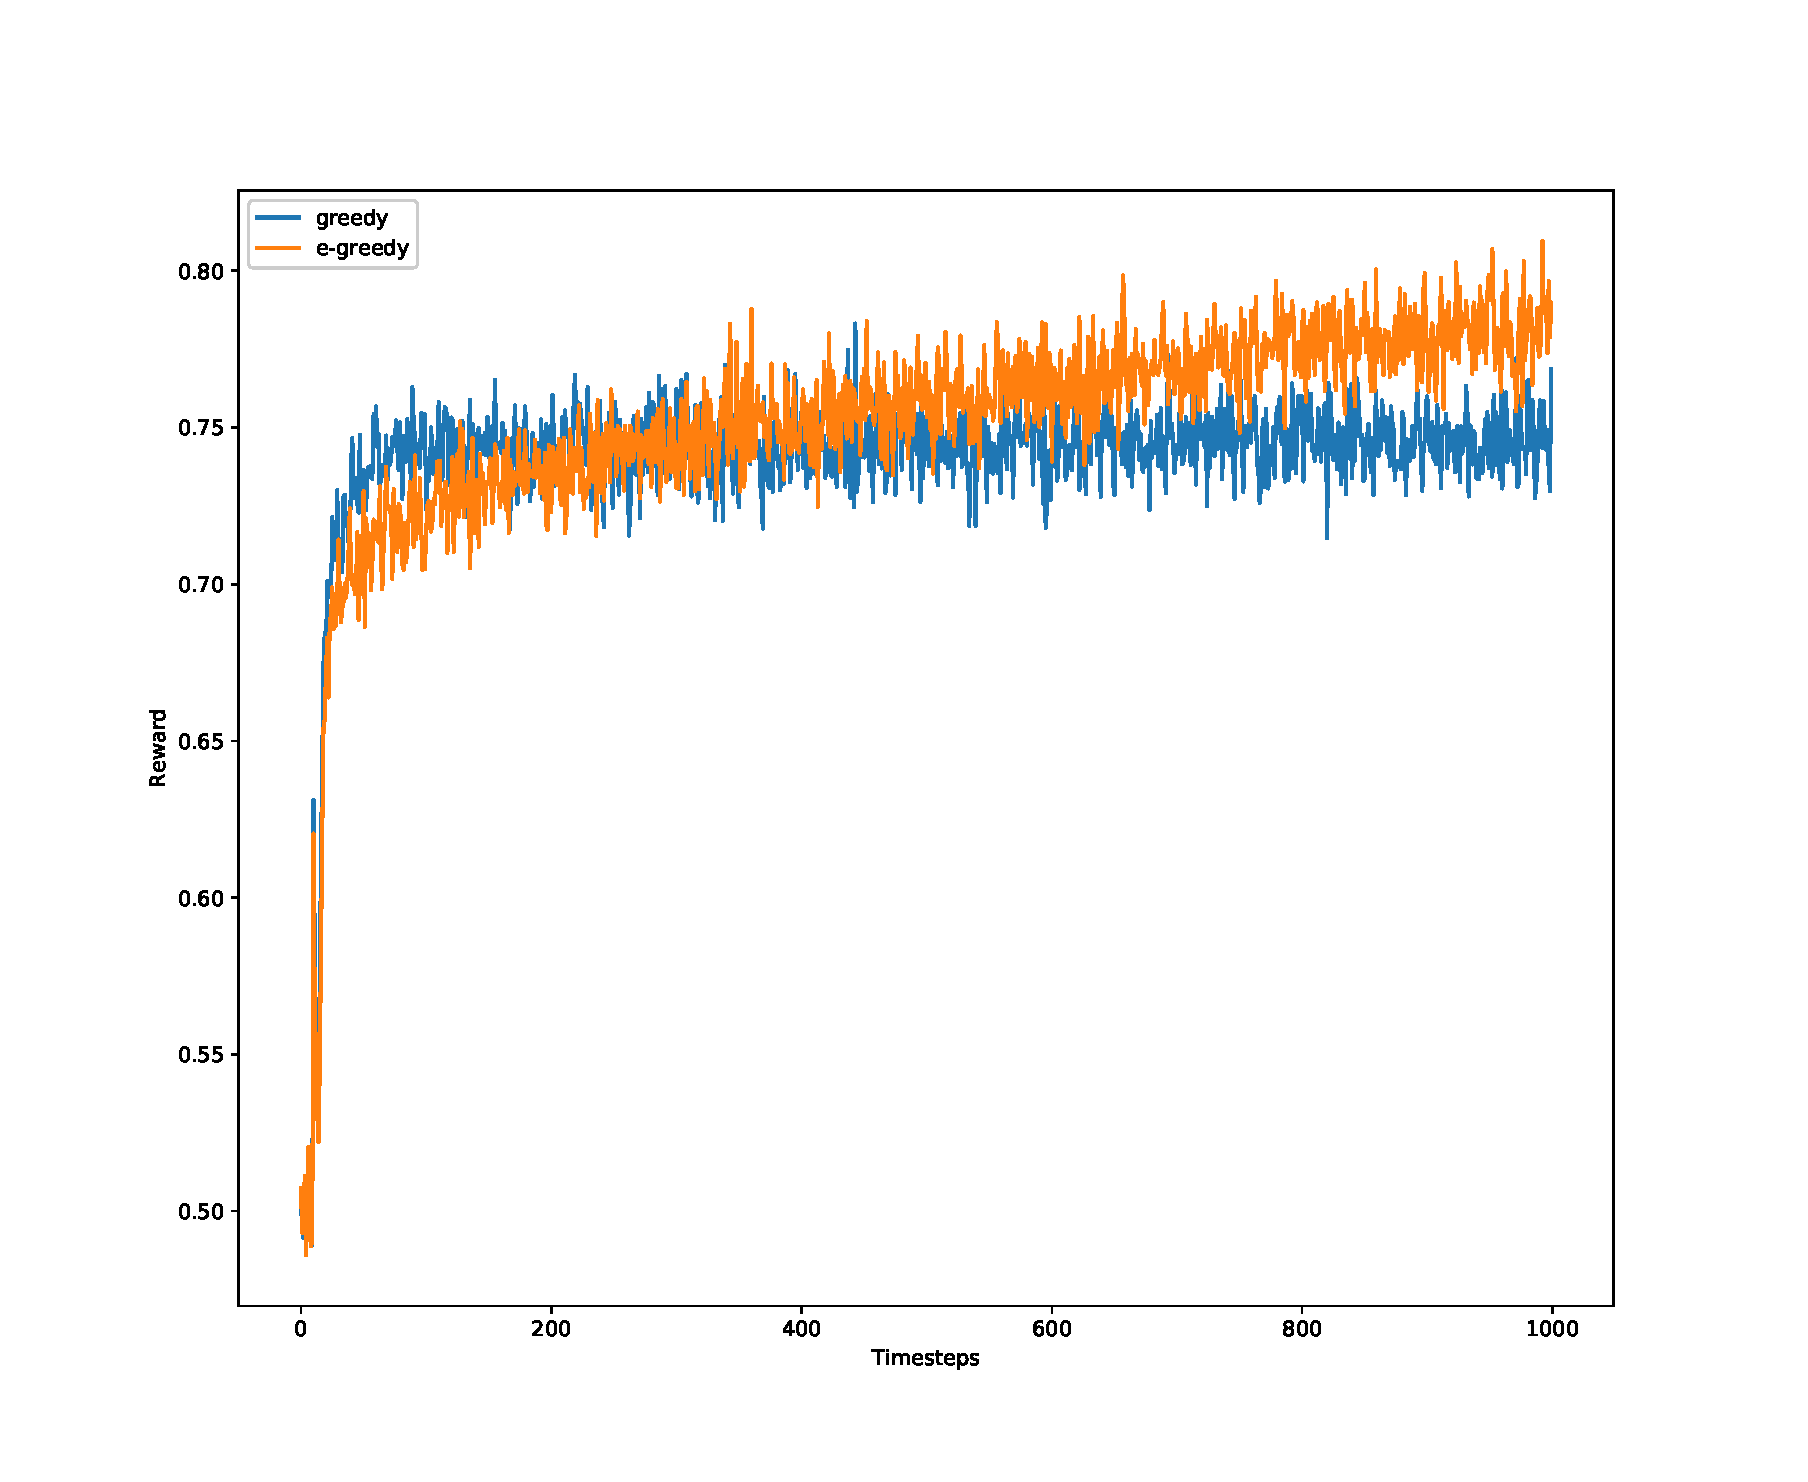
\includegraphics[width=.7\textwidth]{fig_esp_greedy.eps}
    \centering
    \caption{plot of the greedy (blue) and the $\epsilon$-greedy (orange) policy}
    \label{fig1}
\end{figure}

\subsection{}

It might be useful to be more explorative in the beginning of our runtime to while being more exploitive 
the nearer we get to the end of our trials. This way we are more likely to find the most rewarding 
action(s) at the start and maximize our total reward towards the end. \newline
This stratety would be especially useful for cases were we don't have that many trials. \newline
For example we can start with a higher $\epsilon=0.5$ than before and slowly converge to an $\epsilon=0$ strategy
during the first half of our trials. This way we end up with a high rewarding exploitive-only policy for the 
second half of our trials: \newpage

\begin{center}
    \begin{lcverbatim}
        eps = 0.5
        eps_add = float(0.5/(timesteps*0.5))

        while bandit.total_played < timesteps:
            if bandit.total_played < (timesteps*0.5):
                if random.random() < (eps - bandit.total_played*eps_add):
                    a = random.randint(0,(bandit.n_arms-1))
                else:
                    a = np.argmax(Q)
            else:
                a = np.argmax(Q)
    \end{lcverbatim}
\end{center}


\flushleft As you can see in in figure \ref{fig2} this leads to less rewards in the beginning, but performes better
than the previous methods after some time. We end up with an higher total reward of $782.67$ compared with $753.98$ for the
$\epsilon$-greedy policy and $734.54$ for the greedy-only strategy.

\begin{figure}[h!]
    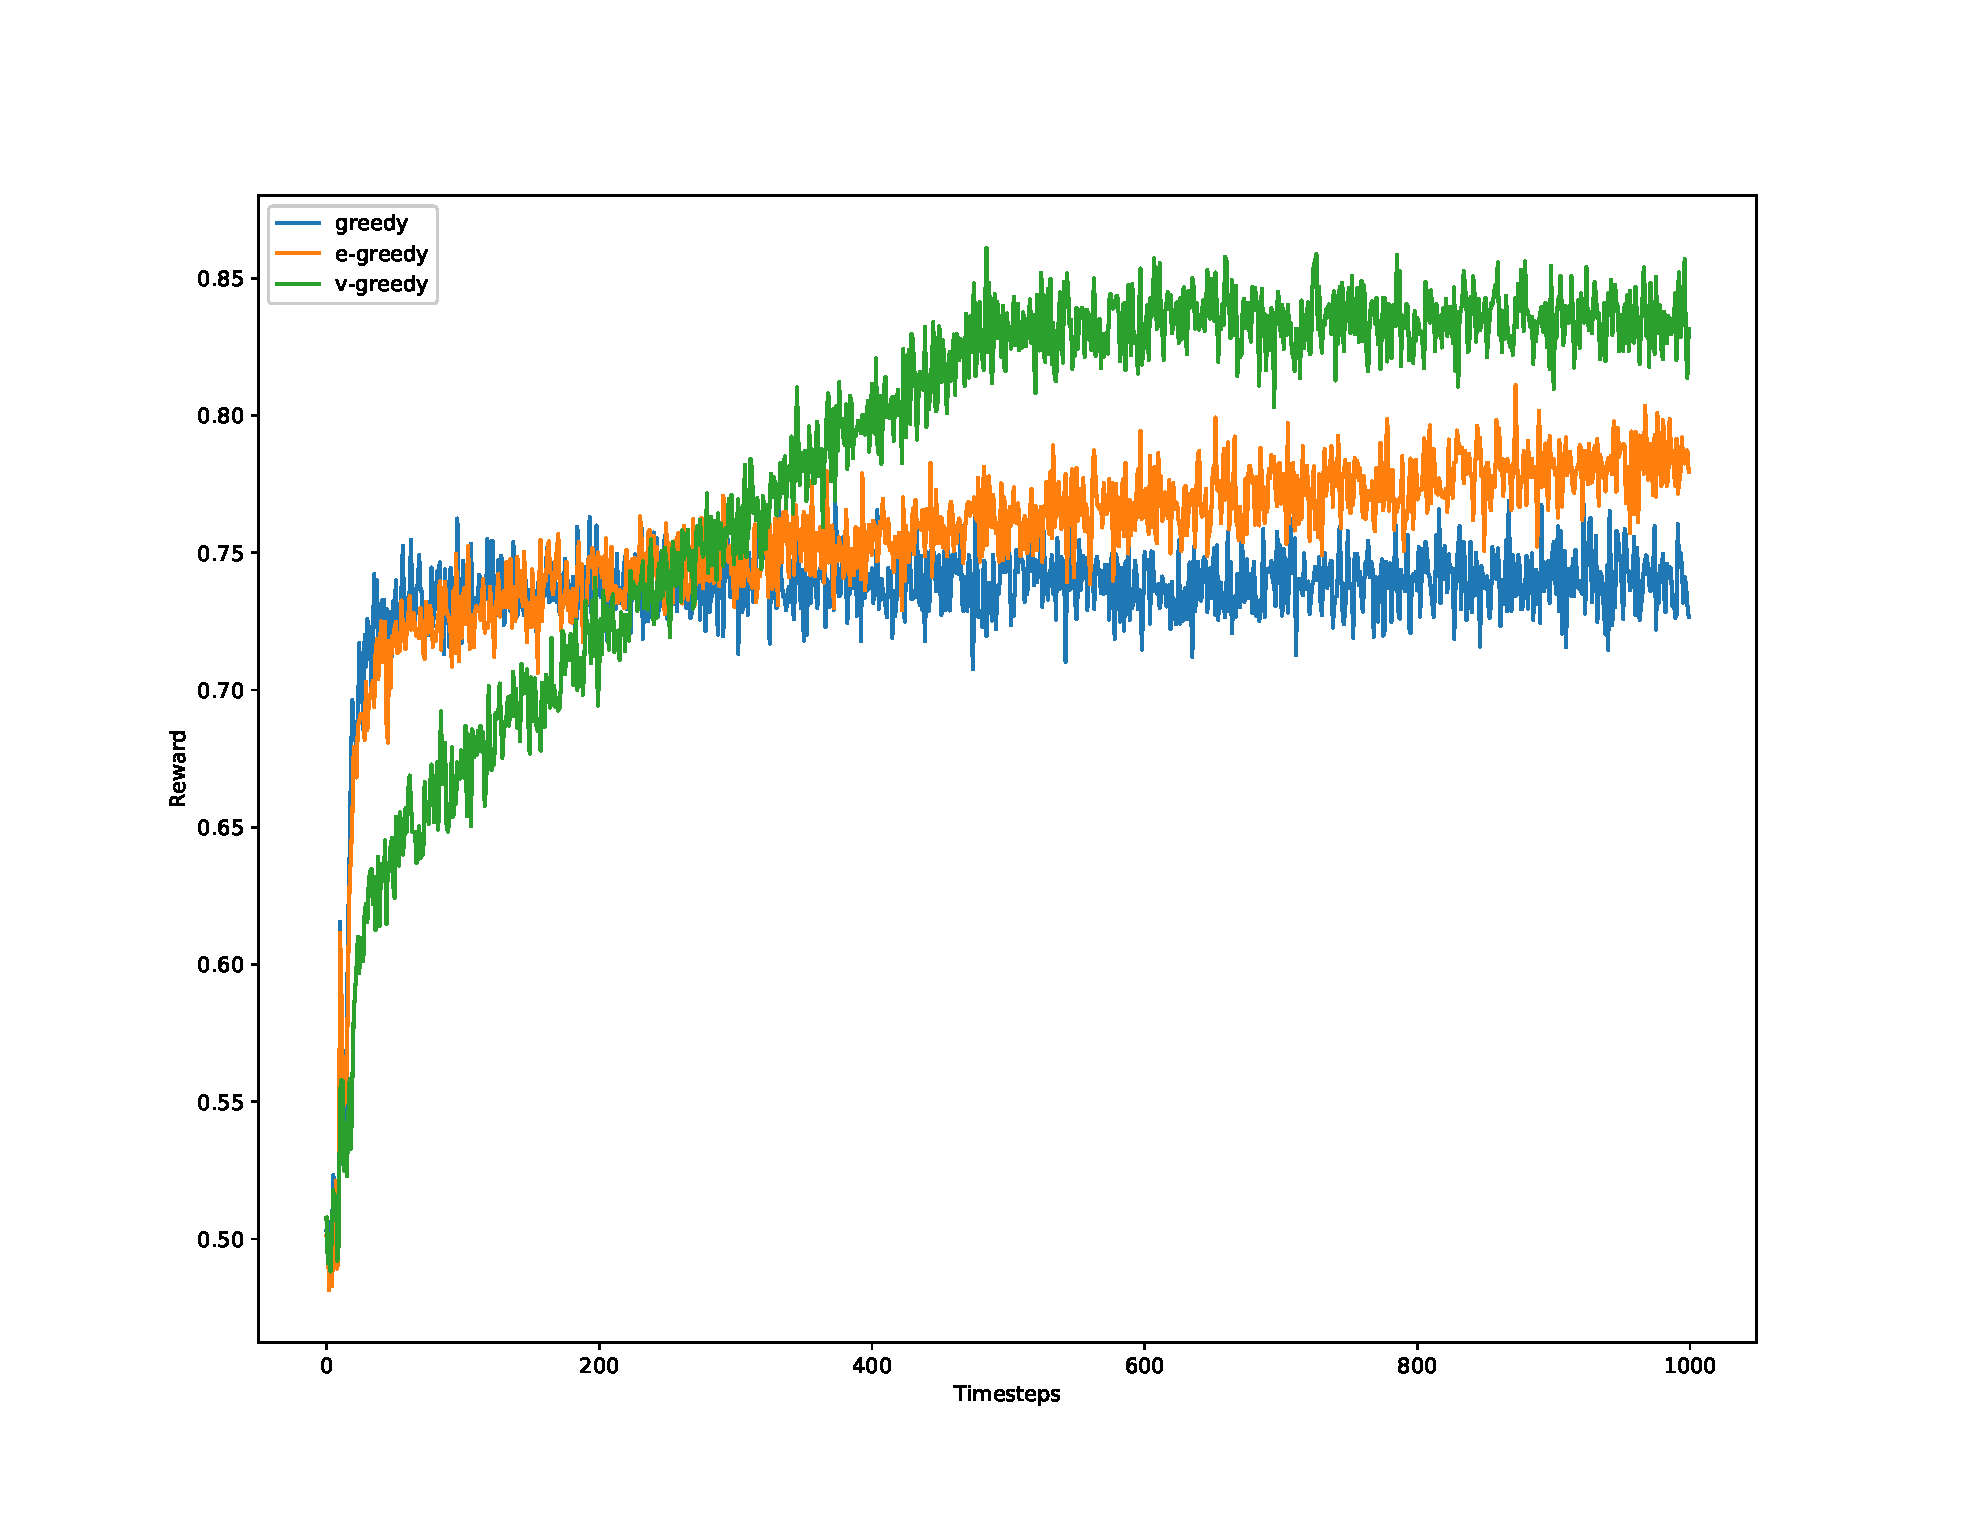
\includegraphics[width=.7\textwidth]{fig_experimental_3.eps}
    \centering
    \caption{plot of the strategy with decreasing explorativity (green) compared with the previous methods}
    \label{fig2}
\end{figure}



\end{document}